
\section{Computing for Energy Frontier Science}

In an attempt to get a reasonable prediction of the magnitude of
changes that could be expected from a new program in the next ten
years, we look back on the changes between the Tevatron and LHC over
the last 10 years.  In 2003 the Tevatron was in the 3rd year of Run2
and comparing it to the third year of LHC in 2012 there is a rough
factor of 10 in the metrics associated with data acquisition and event
complexity as can be seen in Table~\ref{tab:compare_daq}. In addition
to the data acquired, the computing scales with the collabroation and
activity needs and those metrics are shown in
Table~\ref{tab:compare_coll}.

\begin{table}[t]
\begin{center}
\begin{tabular}{lll}
Metric & Tevatron (2003) & LHC (2012) \\ \hline
Trigger rate & 50Hz & 500Hz \\
Prompt Reconstruction rate/week & 13M Events & 120M events \\
Re-reconstruction rate & 100M events per month & 800M - 1B events per month \\
Reconstructed size & 200kB & 1-2MB \\
AOD size & 20kB & 200-300kB \\
Reconstruction time & 1-2s on CPUs of the time & \~ 10s on CPUs of the time \\ \hline
\end{tabular}
\caption{Relevant data acquisition and complexity metrics comparing Tevatron and LHC at similar points.}
\label{tab:compare_daq}
\end{center}
\end{table}


\begin{table}[t]
\begin{center}
\begin{tabular}{lll}
Metric & Tevatron (2003) & LHC (2012) \\ \hline
Collaboration Size & 800 & 2000-3000 \\
Number of individual analysis submitters per day & 100 & 300-400 \\
Number of total analysis submitters & 400 & Greater than 1000 \\ \hline
\end{tabular}
\caption{Relevant collaboration and participation metric comparing Tevatron and LHC at similar points.}
\label{tab:compare_coll}
\end{center}
\end{table}

Combining the increase in complexity, which is reflected in event size
and reconstruction time, with the increases in physics triggers and
the improvements in computing technology the total capacity increase
is much larger.  The globally distributed nature of LHC computing,
which includes the majority of the computing capacity located away
from the host lab, places much higher expectation on the networking
and data handling.  Both of these effects can be seen in
Table~\ref{tab:compare_comp}.

\begin{table}[t]
\begin{center}
\begin{tabular}{lll}
Metric & Tevatron (2003) & LHC (2012) \\ \hline
Remote Computing Capacity & 15kHS06 (DZero Estimated) & 450kHS06 (CMS) \\
User Jobs launched per day & 10k per day & 200-300k jobs per day \\
Disk Capacity per experiment in PB & 0.5PB & 60PB \\
Data on Tape per experiment  & 400TB & 70PB \\
MC Processing Capacity per month for Full Simulation & 3M & 300M \\
Data Served from dCache at FNAL per day & 25TB & 10PB \\
Wide Area networking from host lab & 200Mb/s & 20000Mb/s \\
Inter VO transfer volume per day & 6TB (DZero SAM) & 546TB (ATLAS) \\ \hline
\end{tabular}
\caption{Relative capacity comparisons between Tevatron and LHC at similar points.}
\label{tab:compare_comp}
\end{center}
\end{table}


The processing capacity between the 2 programs has increased by a
factor of 30, which is almost exactly what would be expected by the 2
year Moore's law doubling cycle.  This is also reflected in the number
of user jobs, which will normally expand to fill the available
resources.  The disk capacity, the local data served, the wide area
networking from the host lab, and the inter-site transfers are all
increased by a factor of 100.  This is caused by the change in
computing model to have a much high degree of distribution, but even
more impacted by the factor of 10 increase in trigger rate and the
factor of 10 increase in event size.  The full event simulation
capacity is also 100 times larger in the LHC program, which may
indicate the larger importance of simulation.  The factor of 30
increase in processing with a factor of 100 increase in IO and storage
makes an argument that processing scales as what can be accommodated
by Moore's law, and storage and IO scale with trigger rate and event
size.  The LHC has been successful even though these two numbers have
not increased at the same rate, but points toward the effort expended
in making efficient code and points toward issues facing computing for
the energy frontier moving forward.

The increase in LHC computing and disk storage is shown in
Figure~\ref{fig:growth}.  The CPU increases at a rate of 363kHS06 per
year and the disk at 34PB a year on average.  The rough linear
increase is the combination of three separate periods that average to
linear.  The period 2008, 2009, and 2010 were the procurement ramp for
LHC as the scale of the available system was tested and commissioned.
The period from 2010 to 2013 is the first run where the computing and
storage increased at a rate defined by the incoming data to process
and analyze.  The resources needed to accommodate the higher trigger
rate and event complexity expected in the second run define 2015.  The
three periods roughly average out to a linear increase.

In energy frontier computing data tends to be analyzed intensively at
the beginning and then archived and accessed less as most of the
relevant results are gleaned from the data in the first few years
after collection.  Therefore, the growth curves below do not scale
with total integrated luminosity but indicate that more inputing is
needed per unit time as trigger rates and event complexity increase.
It is not reasonable to expect that the techniques currently used to
analysis data in the energy frontier will continue to scale
indefinitely.  The energy frontier will need to adopt new techniques
and methods moving forward.

%%%%%%%%%%%%%%%%%%%%%%%%%%%%%%%%%%%%%%%%%%%%%%%%%%%%%%%%%%%%%%%%%%%%%%%%%
%%
%%   use this format to include an .pdf figure into your paper
%%
\begin{figure}[htb]
\begin{center}
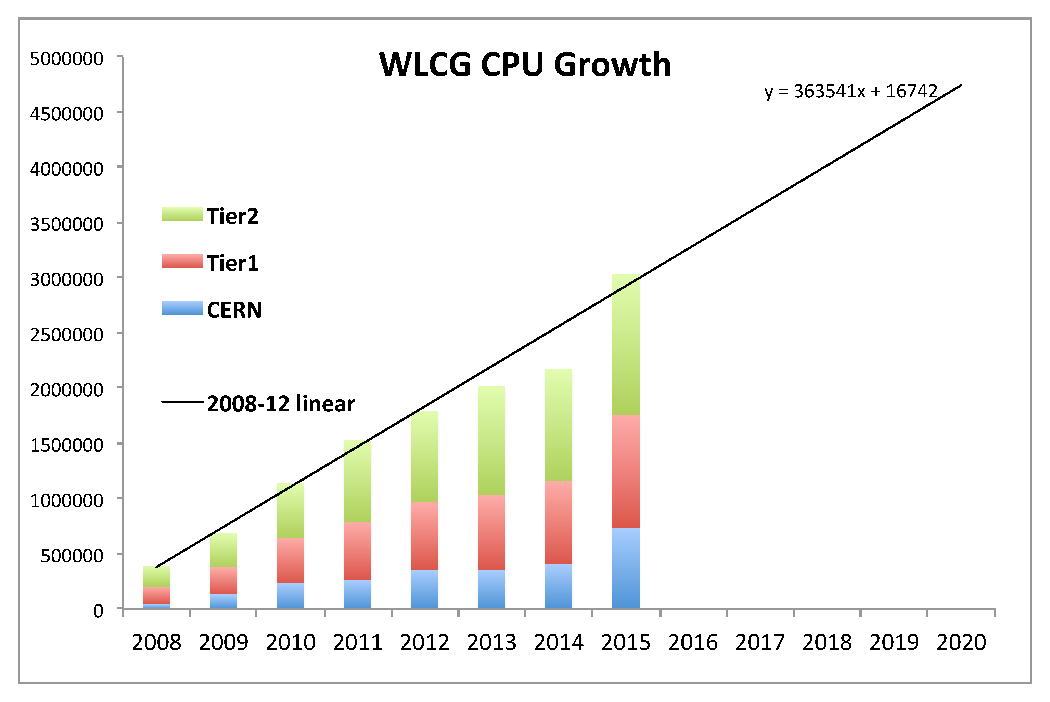
\includegraphics[width=0.45\hsize]{CpF-E2/Growth1.eps}
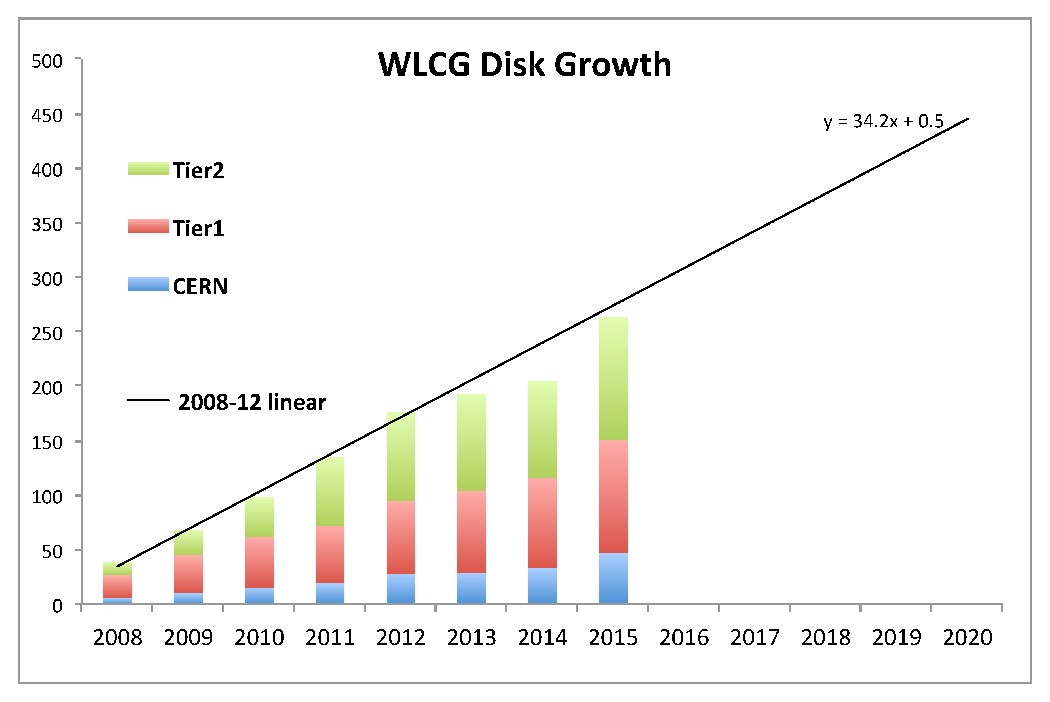
\includegraphics[width=0.45\hsize]{CpF-E2/Growth2.eps}
\caption{Shows the CPU and disk growth through the first 7 years of the program.}
\label{fig:growth}
\end{center}
\end{figure}
%%%%%%%%%%%%%%%%%%%%%%%%%%%%%%%%%%%%%%%%%%%%%%%%%%%%%%%%%%%%%%%%%%%%%%%%%%%



If we extrapolate out 10 years, LHC computing would have roughly 3
times the computing expected in 2015, which is much lower than Moore's
law doubling expectations.  LHC would reach nearly 800PB of disk by
2023, which is again roughly a factor of 3 over 2015.  The LHC numbers
are probably sustainable with this rates and budgets that are close to
flat for computing.  There are potential efficiency improvements and
new techniques that will be discussed below.  More concerning is a
potential new program like a Super LHC, an ILC, or a LEP3 where the
luminosity or complexity increases dramatically and computing is not
on the curve in Figure~\ref{fig:growth}, but is a shift like the
difference between Tevatron Run2 and LHC Run1.  The proposed changes
below will potentially help make better use of the computing available
for LHC, and will be critical as Energy Frontier machines begin to
have data rates and conditions that would be expected in intensity
frontier computing.

